\documentclass[a4paper, 12pt]{article}
\usepackage{fullpage}
\usepackage[utf8]{inputenc}
\usepackage[english]{babel}
\usepackage{latexsym}
\usepackage{color}
\usepackage{amssymb}
\usepackage{amsmath}
\usepackage{graphicx}
\usepackage{fancyhdr}
\usepackage{subfigure}

\pagestyle{fancy}
\fancyhf{}
\fancyhead[RE,LO]{Project 2: Learning of Grid Cells}
\headsep=15mm

\title{Project 2: Learning of Grid Cells}
\author{Claus Lang, Can Eren Sezener, Claudia Winklmayr}
\date{09.02.2016}


\begin{document}
\maketitle

\paragraph{Abstract:}
Grid cells, located in rats medial entorhinal cortex (mEC), show increased firing activity when the animal enters specific regions of the environment. The resulting firing maps show a characteristic hexagonal grid pattern. In our project we implement a computational model for the development of grid cells, introduced by Kropff and Treves. We simulate a rat exploring a square environment. The $x$ and $y$ coordinates of its locations serve as input for a layer of 40 place units. The output layer then receives a weighted sum of the places cell activity to compute the grid cell activation. Weights are updated by a Hebbinan learning rule. 

\section{Introduction}
There are various types of neurons that serve to encode an animals spacial location. Place cells- located in hippocampus- were discovered in the 1970s by O'Keefe and Dostrovsky. Place cells show increased activity when the animal enters a specific region of the environment- the so called place field.\newline
Grid cells - located in medial entorhinal cortex (mEC) were then discovered in 2005. In contrast to place cells they are activated at various locations and their firing maps show a characteristic hexagonal grid pattern. Different grid cells can be distinguished by their spacing, orientation and spacial phases and neighboring grid cells show similar and orientation. \newline
It is assumed that grid cells perform a path integration task, taking into account the rats position, speed and direction. Visual information on the other hand plays at most a secondary role in the formation of the grid pattern. \newline
The Kropff and Treves model assumes places cells as the basis for grid cell development. The place cells take as input the $x$ and $y$ coordinates of a virtual rat exploring a square environment of 125cm length. Every output unit then receives input from all place cells and the weights connecting input and output neurons are updated by a Hebbian learning rule. 
%
%
%
\section{Model}
%
%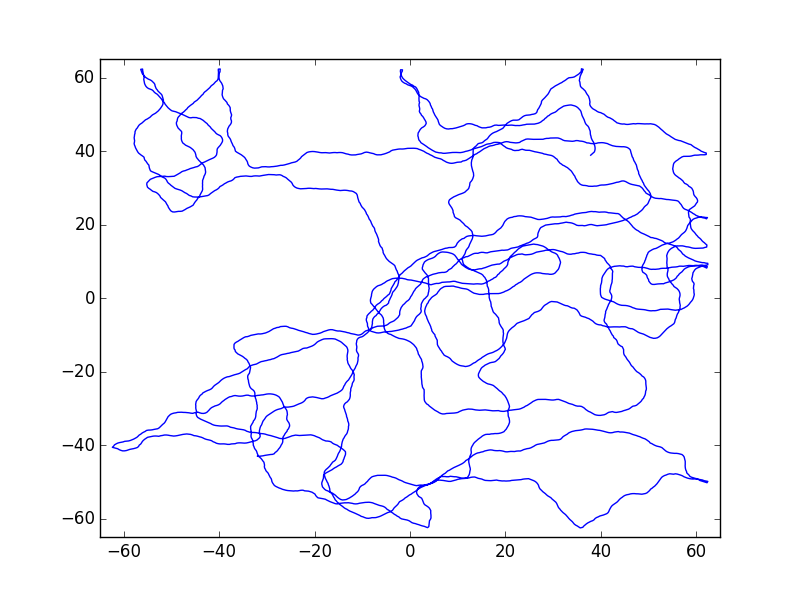
\includegraphics[width=6cm]{running_rat.png}
%\caption{running time: 50 seconds}


%
%
%
\section{Results}
We ran the simulation for 2.5 hours in rat time. The results show that this duration is sufficient for grid cells to develop. Figure \ref{time-evol} shows the time evolution of weights of a grid cell. The cell we picked has one of the most apparent grid structure among the other cells.

%\subsection{Time evolution}
\begin{figure}[htbp]
\begin{minipage}[hbt]{0,49\textwidth}
        \centering
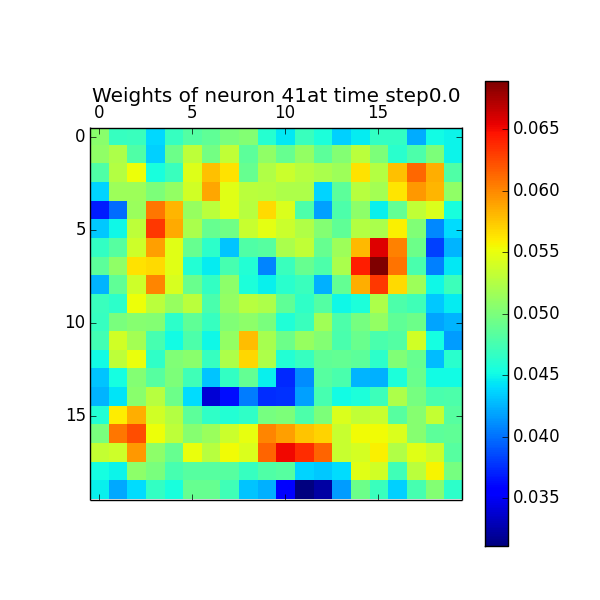
\includegraphics[width=6cm,height=6cm]{neurons/neuron_w_41_t_0.png}\\[10pt]
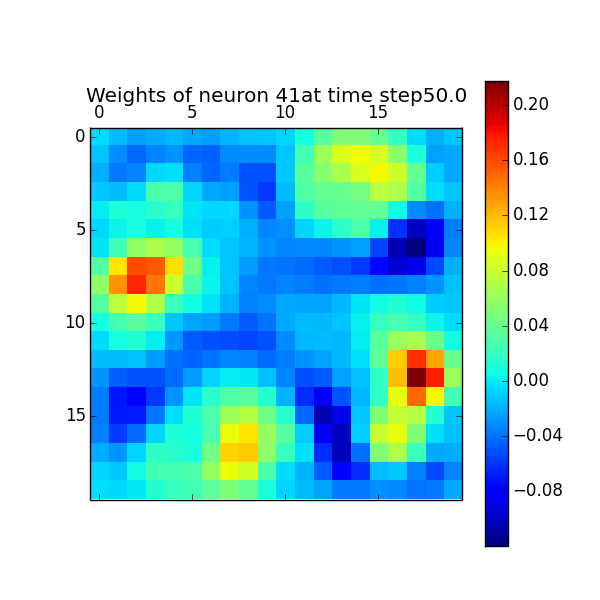
\includegraphics[width=6cm,height=6cm]{neurons/neuron_w_41_t_50.png} \\[10pt]
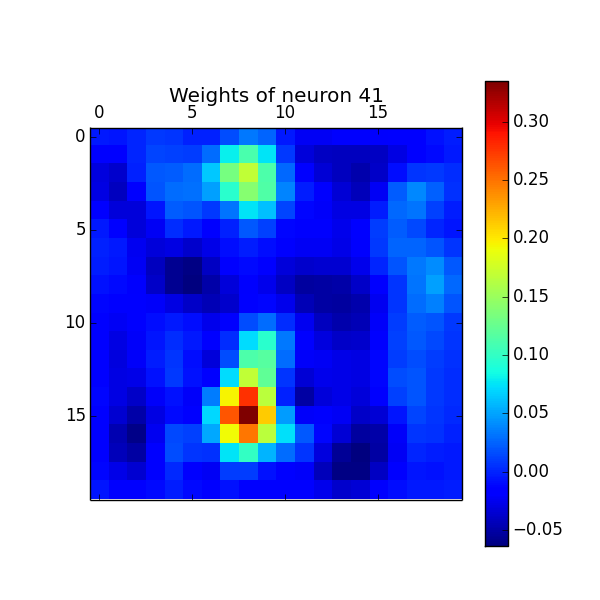
\includegraphics[width=6cm,height=6cm]{neurons/neuron_w_41.png}
        \caption{weight development}
        \label{LabelA}
\end{minipage}
\begin{minipage}[hbt]{0,49\textwidth}
        \centering
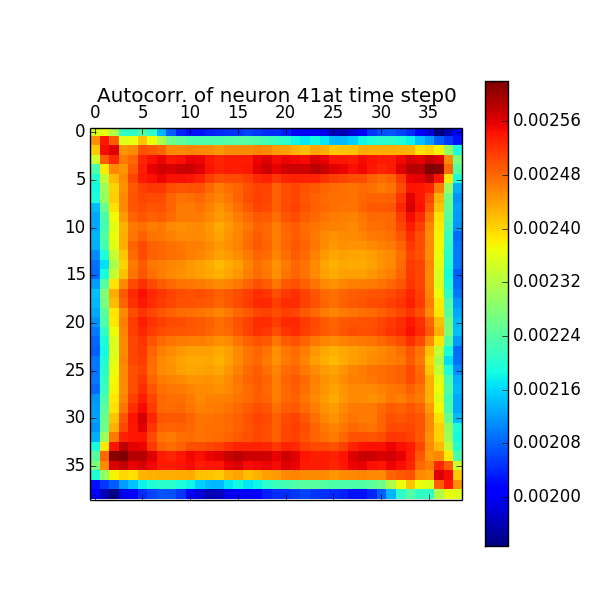
\includegraphics[width=6cm,height=6cm]{neurons/neuron_a_41_t_0.png}\\[10pt]
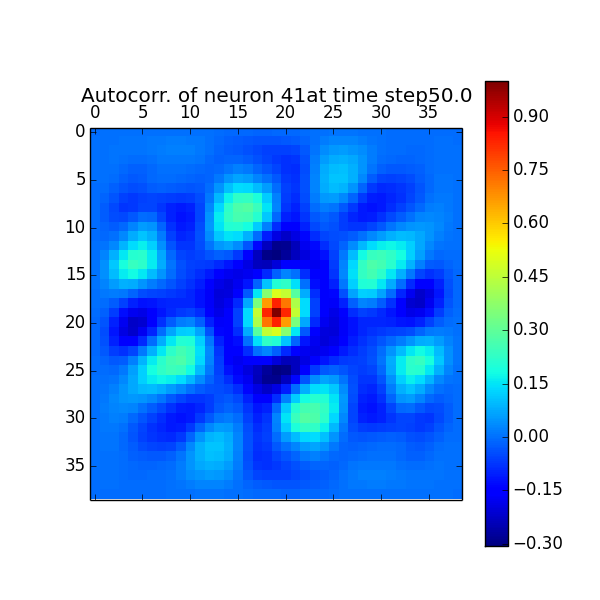
\includegraphics[width=6cm,height=6cm]{neurons/neuron_a_41_t_50.png}\\[10pt]
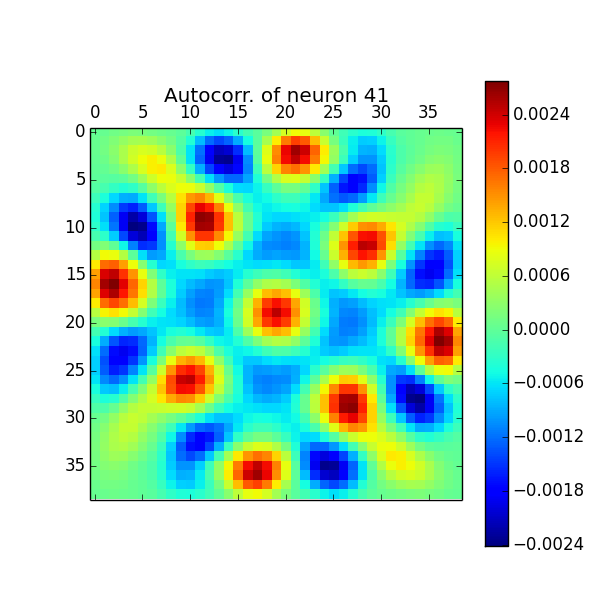
\includegraphics[width=6cm,height=6cm]{neurons/neuron_a_41.png}
        \caption{autocorrelation development}
        \label{LabelB}
\end{minipage}
\centering
\caption{The weights and the autocorrelogram of a neuron at the beginning, middle and the end of the simulation}
\label{time-evol}
\end{figure}

When all grid cells are inspected, it is seen that most grid cells have similar spatial frequencies, however, their orientations and off-sets are different. Figure \ref{diff} illustrates this difference. 

\begin{figure}
\hfill
\subfigure{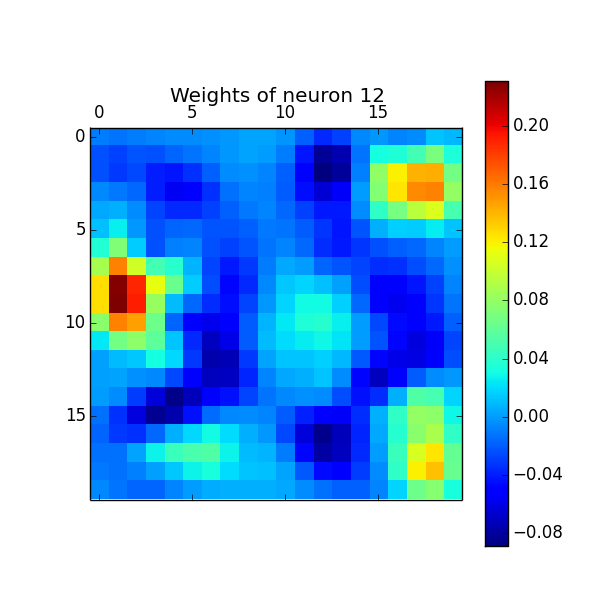
\includegraphics[width=6cm]{neurons/neuron_w_12.png}}
\hfill
\subfigure{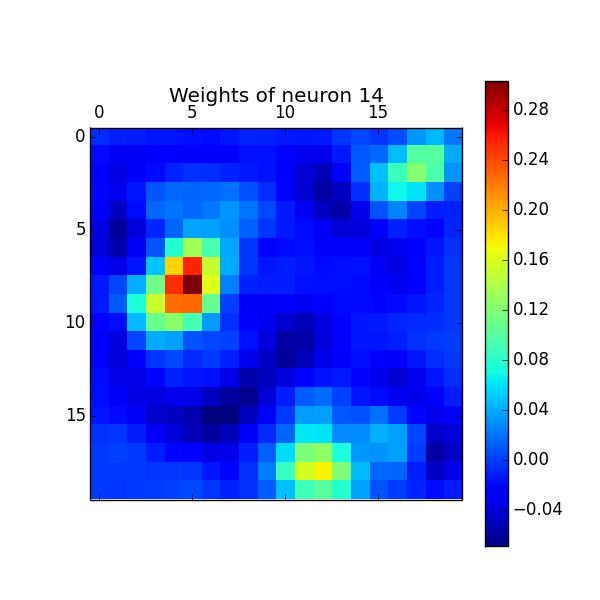
\includegraphics[width=6cm]{neurons/neuron_w_14.png}}
\hfill
\caption{Different grid cells have different orientations and off-sets but similar spatial frequencies.}
\label{diff}
\end{figure}

\section{References}

\end{document}

	